%\graphicspath{{images/chap4/}}


\section{Assembly Standards}
\epigraph{The following sections were written by members of the Sorbonne team}{\textit{iGEM Sorbonne\_U\_Paris 2021}}
\noindent
One of the major characteristics of synthetic biology is the ease with which we can build genetic networks. Assembly standards can be defined as the set of rules followed by the engineer to assemble bio bricks. For more than fifteen years, in vitro DNA assembly was limited by the use of digestion, ligation and restriction enzymes. Nowadays, assembly standard uses a combination of restriction sites to enable the insertion of new biological parts while conserving both the beginning and the end of the genetic sequence. To ensure rapid implementation and reproducibility, it is important to standardized assembly protocols. The fewer rules the assembly will have, the easier it will be to apply, guaranteeing a smaller toolbox and a lower price. \\ \\
The first widely adopted standard in synthetic biology was the BioBrick. All Biobricks are flanked between sequences called prefix and suffix2. These sequences include restriction sites, which is where the restriction enzymes will make their cut. Plasmid cleavage generates sticky ends, which will come together and facilitate the ligation between BioBrick parts. Indeed, the goal of assembly standards is to fuse protein coding domains. Thanks to this process, multiple Biobrick parts can be assembled and it results in a more complex system than the original one. \\ \\
There are different types of assembly standards, which differ by the prefix and suffix sequences and the restriction sites they contain. Assembly standards also generate a scar sequence (yellow sequence in Figure 4.1), which corresponds to the sequence between the fused BioBricks and depends on part type. 

\begin{figure}[!htbp]
    \centering
    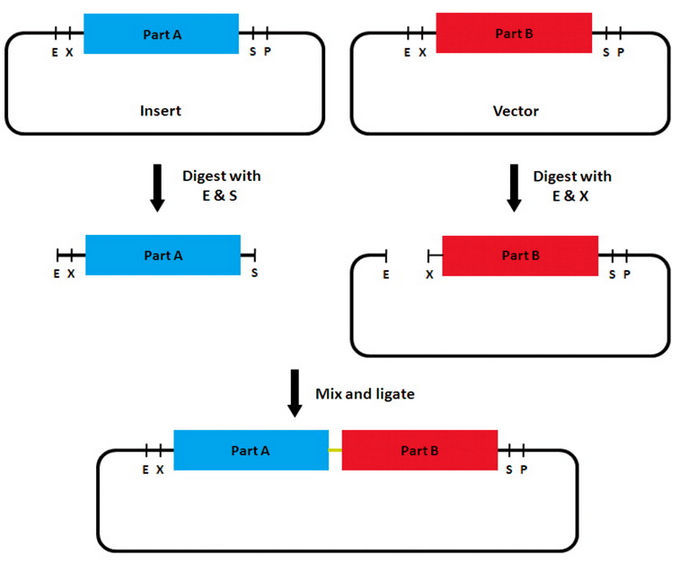
\includegraphics[width=0.8\textwidth]{images/chap4/chap4_asm_01.png}
    \caption{Standard assembly of two BioBricks (part A and part B)3. The part A plasmid is digested with EcoRI (E) and SpeI (S), the part B plasmid is digested with EcoRI (E) and XbaI (X). The sticky ends are compatible for ligation and the two parts can be assembled.}
    \label{fig:ch4asm01}
\end{figure}
\FloatBarrier
\noindent
The most significant quality of an experiment standard is its idempotency, which means that it should result in the same effect every time you apply it and that any newly added part will adhere to its assembly. \\ \\
To build complex genetic circuits, the toolkit should present a large diversity of parts to provide maximum modularity to the user, as you can see in Figure 4.2. 

\begin{figure}[!htpb]
    \centering
{{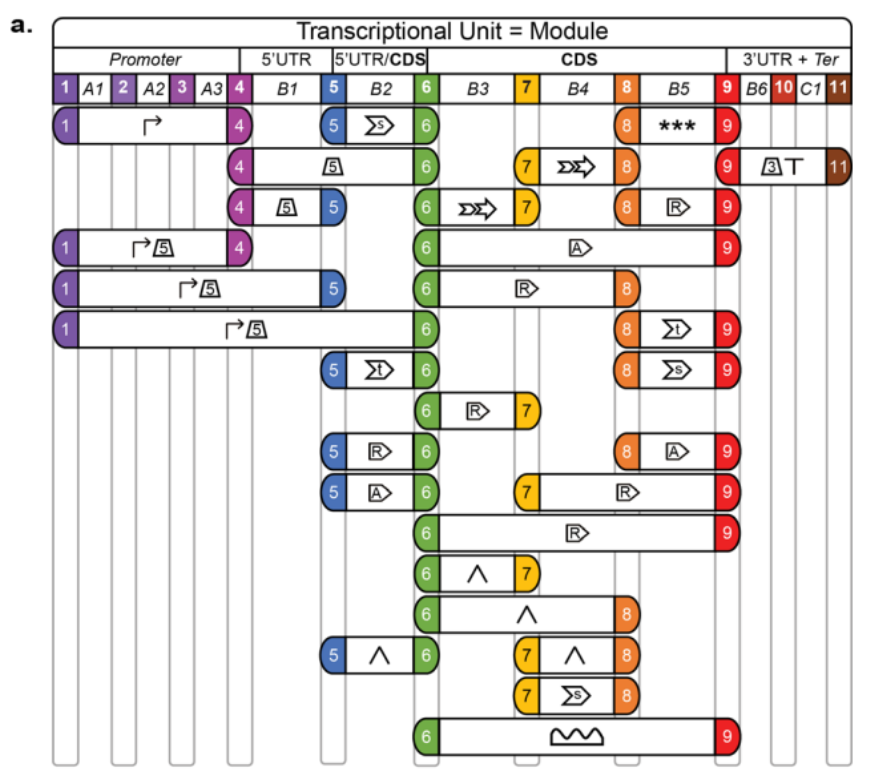
\includegraphics[width=10cm]{images/chap4/chap4_asm_02.png} }}%
    \qquad
{{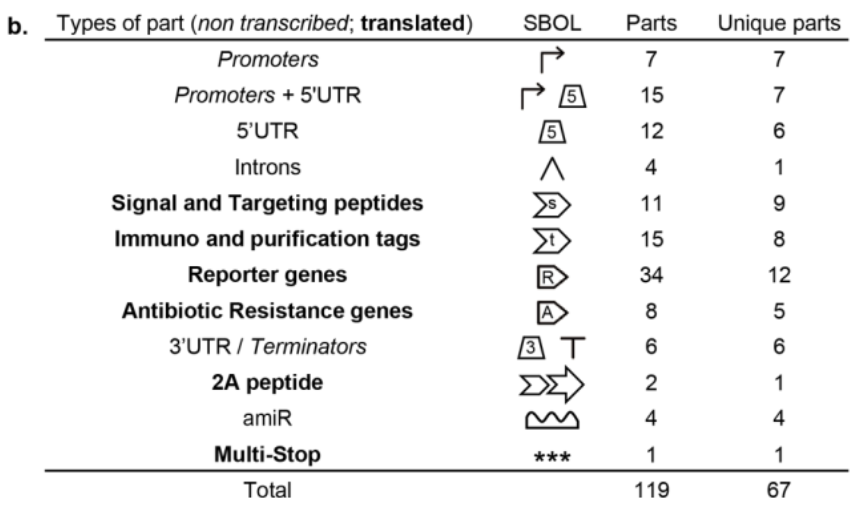
\includegraphics[width=10cm]{images/chap4/chap4_asm_03.png} }}%
    \caption{Standardised genetic parts in the \textit{Chlamydomonas} MoClo kit}%
    \label{fig:ch4asm02}%
\end{figure}
\FloatBarrier

\noindent Today, among all standardized tools, the Golden Gate Modular Cloning (MoClo) is widely used. MoClo is based on the exploitation of type II restriction enzymes to construct complex DNA sequences in only two steps. Type IIS assembly methods have been widely adopted in plant research laboratories but also for the engineering of fungi. These enzymes have the particularity to cut a few nucleotides after their recognition site. The idea is to get together multiple plasmids, each one containing one part of the gene assembly and, using only one Type II enzyme, obtain the final assembly in one step. 

\section{PhytoBricks}
\epigraph{The following section was written by Michael Burgis}{\textit{iGEM Marburg 2021}}
\subsection*{Standardization in Phototrophic Synthetic Biology}
The standardization of components in common engineering disciplines, from screw threads to printed circuit boards, is one of the key elements to facilitate both the speed of innovation and the economy of production processes. \\
The introduction of standards, in particular for the DNA assembly of characterized DNA sequences, was a landmark in microbial engineering, which heavily shaped the emerging field of synthetic biology in its early days . \\ \\
In order to facilitate the easy exchange of standardized genetic parts in plant and phototrophic chassis , the international plant science community established a common genetic syntax for DNA parts \parencite{Patron2015}. This standard is based on Type IIS restriction enzymes and enables parallel assembly of multiple DNA parts in a one-pot, one-step reaction, called Golden Gate assembly. \\ \\
Before the agreement of the  Phytobrick standard, many labs have started their own standardisation efforts by converting in house plasmids to the use of Golden Gate cloning. The GoldenBraid2.0 (GB2.0) and Golden Gate Modular Cloning (MoClo) assembly standards, which are described later in this handbook, have been adopted by the plant research communities and are partly, but unfortunately not entirely compatible.  Even small variations in the different standards prevent the exchange of parts between labs and hinder the creation of a collection of standardized, characterized, exchangeable parts for phototrophic chassis. \\ \\
The standard syntax, calles Phytobrick standard, which we would like to introduce here now, addresses exactly that, by establishing a common grammar to enable the sharing of parts throughout the plant science community, by being compatible with the most widely adopted Type IIS-based standards.

\subsection*{The Phytobrick syntax for phototrophic chassis}
The first rule of the Syntax is that all internal instances of the Type IIS restriction enzyme recognition sequence must be removed and subsequently the part has to be cloned into a compatible backbone, flanked by Type IIS restriction enzyme recognition sequences. This Backbone should also be free of the mentioned typeIIS recognition sides and additionally should also not contain bacterial resistance to ampicillin/carbenicillin or kanamycin as these are commonly utilized in the plasmids in which standard parts will be assembled into. This process is called domestication. When released from its plasmid backbone by the restriction digest with BsaI, each part contains specific, four-base-pair overhangs, known as fusion site (Figure 4.3).

\begin{figure}[!htbp]
    \centering
    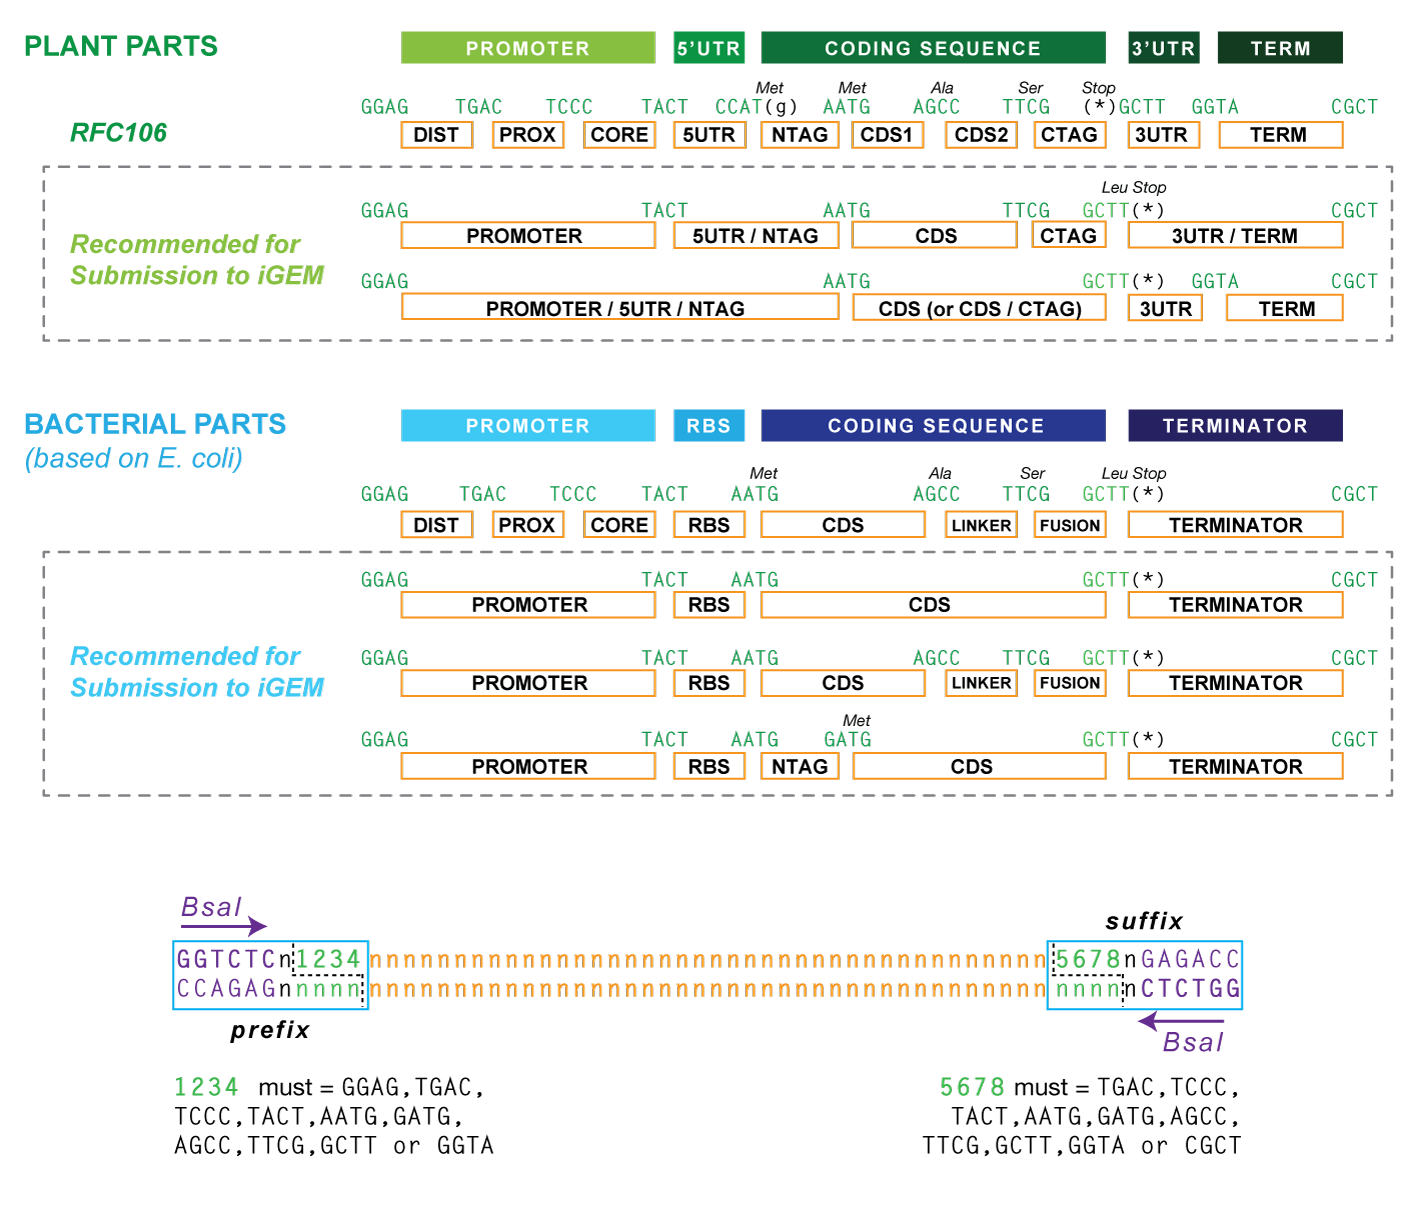
\includegraphics[width=\textwidth]{images/chap4/chap4_phy_01.png}
    \caption{Specific fusion sites of the Phytobrick syntax for the individual part types.}
    \label{fig:ch4phy01}
\end{figure}
\FloatBarrier

\noindent
A standard syntax for transcriptional units has been defined and 12 fusion points assigned. \\ \\
In both systems transcriptional units can be assembled and used directly or may be assembled with other transcriptional units to make multigene assemblies. 


\section{BioBrick RFC[10]}
\epigraph{The following section was written by Michael Burgis}{\textit{iGEM Marburg 2021}}
The Biobrick RFC[10] assembly standard was originally developed by Tom Knight was one of the most widely used assembly standards and still the majority of parts in the iGEM registry database are RFC[10] compatible, which means that they don´t contain illegal recognition/cutting sites for the restriction enzymes of this assembly standard.\\ \\
Additionally all BioBricks are flanked by standardized restriction sites, consisting of the \textbf{BioBrick} \textbf{Prefix} and \textbf{Suffix}. The Biobrick prefix contains the \textbf{E}coRI and \textbf{X}baI cutting sites, flanking the part on the left side and the Biobrick Suffix  includes \textbf{S}peI and \textbf{P}stI on the right.

\begin{figure}[!htbp]
    \centering
    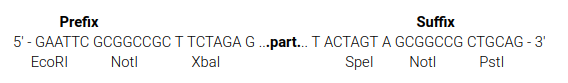
\includegraphics[width=\textwidth]{images/chap4/chap4_bio_01.png}
    \label{fig:ch4bio01}
\end{figure}
\FloatBarrier

\noindent\textbf{There is a second prefix designed for protein coding regions, because of RBS issues!}:

\begin{figure}[!htbp]
    \centering
    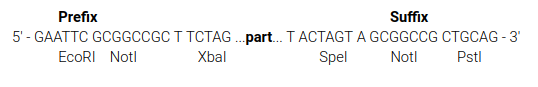
\includegraphics[width=\textwidth]{images/chap4/chap4_bio_02.png}
    \label{fig:ch4bio02}
\end{figure}
\FloatBarrier
\noindent
For the assembly of biobricks several assembly methods have been described. One of them is the 3A assembly (which stands for three antibiotic assembly), which is a method for assembling two BioBrick parts together. It differs from the common Biobrick assembly approach in that it relies on three way ligation (between the two parts and the backbone vector) for assembly rather than two way ligation between a part and a part + vector molecule.
3A assembly was designed such that gel purification of the digested parts is unnecessary,
as gel purification tends to be inefficient especially on small pieces of DNA, is slow and not easily susceptible to automation and scaling.\\ \\
It uses both positive and negative selection to reduce/eliminate the number of incorrect assemblies that give rise to colonies after transformation. One of the basic principles of this assembly method is that the sticky ends of DNA cut with two different restriction enzymes can form scars after successful ligation, which can not be recognized by either of restriction enzymes used in the assembly.\\ \\
Assembling two parts leaves the following scar: 
\begin{center}
5' [part A] TACTAGAG [part B] 3'     
\end{center}
The following description uses BioBrick RFC[10] part samples as an example.
The left part sample is in a plasmid backbone with an antibiotic resistance for antibiotic A.
The right part sample is in a plasmid backbone with an antibiotic resistance for antibiotic B.
A linearized plasmid backbone is selected with neither resistance A nor B. It has AB resistance C. 


\begin{figure}[!htbp]
    \centering
    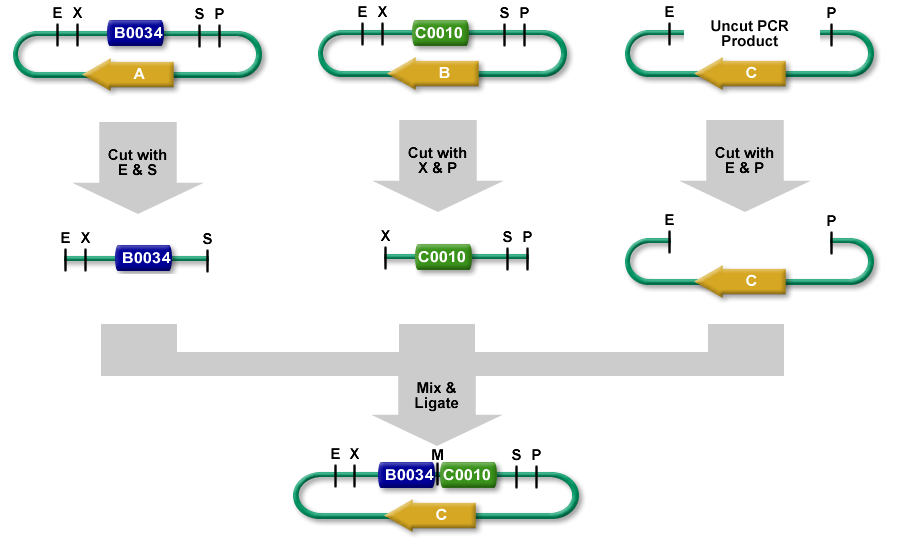
\includegraphics[width=\textwidth]{images/chap4/chap4_bio_03.png}
    \label{fig:ch4bio03}
\end{figure}
\FloatBarrier


\subsection*{Restriction Digests}
The left part sample is cut out with \textbf{E}coRI and \textbf{S}peI. \\ 
The right part sample is cut out with \textbf{X}baI and \textbf{P}stI. \\
The linearized plasmid backbone is cut with \textbf{E}coRI and \textbf{P}stI. \\
All 3 restriction digests are heated to heat kill all of the restriction enzymes. \\ \\
An equimolar quantity of all 3 restriction digest products are combined in a ligation reaction.
The desired result is the left part sample's SpeI overhang ligated with the right part sample's XbaI overhang resulting in a scar that cannot be cut with any of our enzymes. \\
The new composite part sample is ligated into the construction plasmid backbone at the EcoRI and PstI sites. \\
When the ligation is transformed into cells and grown on plates with antibiotic C, only colonies with the correct construction survive. \\ \\
As described above, each cycle of BioBrick/3A assembly joins just two parts together and several rounds of cloning are necessary to construct a full functional transcriptional unit, which is far slower than more recent assembly techniques such as typeIIS based methods or Gibson assembly. Another major concern with BioBrick RFC[10] is that it does not facilitate the assembly of proteins,as the traditional 8bp scar creates a frame-shift, while the alternate 6bp scar includes a stop codon. If you wish to assemble proteins you will want to use an RFC designed specifically for protein assembly.


\section{iGEM Type IIS RFC[1000]}
\epigraph{The following section was written by Yasoo Morimoto}{\textit{iGEM Marburg 2021}}
\subsection*{Introduction}
The iGEM Type IIs assembly provides flexibility and the possibility of a high throughput workflow, it takes advantage of Type IIs restriction enzymes to directionally assemble several genetic parts in a one-pot, one-step reactions. This standard was based on previous works that also put forth similar cloning methods (Moclo, Loop, golden braid). \\ \\ 
Enzymes used: BsaI, SapI \\
Antibiotics used: Chloramphenicol, Kanamycin

\subsection{Type IIS}
Type IIs Restriction enzymes have the special ability to cut outside of their recognition site in a directional fashion, this enables for the selection of arbitrary overhangs and for scarless ligation. \\ \\

\begin{figure}[!htbp]
    \centering
    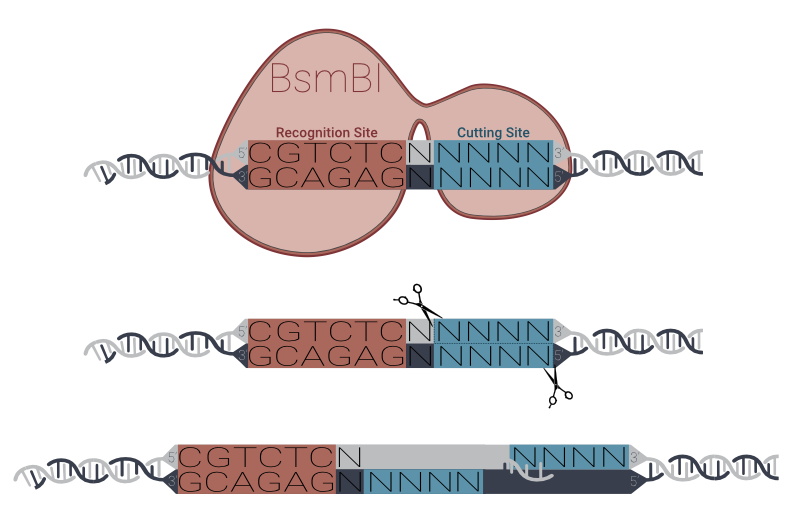
\includegraphics[width=\textwidth]{images/chap4/chap4_rfc1000.png}
    \label{fig:ch4rfc1000}
\end{figure}
\FloatBarrier

 \noindent
The overhangs (fusion sites) used for each part have been standardized for greater interchangeability; Newer Assembly systems have mostly adopted the fusion sites proposed by the MoClo paper \parencite{Weber2011}, therefore, parts in the registry can be used by different systems, given that they don’t contain Illegal cutting sites. RCF 1000 also uses the MoClo fusion sites for its parts. \\ \\
The standard uses the enzymes BsaI and SapI, so compatible parts can’t have these restriction sites insite their sequence. Note that standard compatibility doesn’t depend on the prefix/suffix surrounding the part, those can be arbitrarily chosen depending on the desired assembly system, but if a part has for example a bsaI recognition site (5'...GGTCTC N NNNN...3’) in its sequence, it won’t work in the Type IIS assembly, independently of the prefix/suffix. \\ \\
The assembly process works by successively cloning genetic parts from level 0 plasmids in higher order constructs. Level 1 plasmids take in transcription units (TUs), which can be in turn assembled into Multi-Transcription units (MTUs) in level 2 plasmids.

\subsection*{Level 0}

Parts stored in the level 0 plasmid pSB1C00 can be cut out with BsaI, the fusion sites left on the part are correspondent to the part’s position in the transcription unit:
table of the fusion sites
\begin{figure}[!htbp]
    \centering
    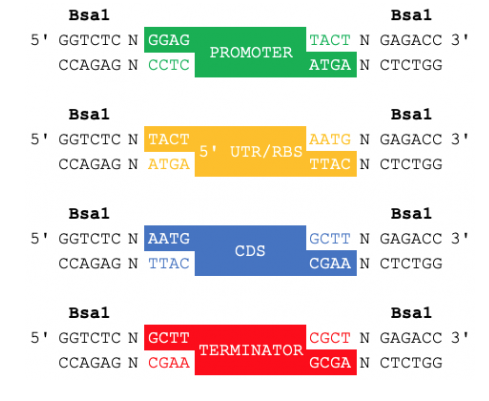
\includegraphics[width=0.8\textwidth]{images/chap4/chap4_typ_01.png}
    \label{fig:ch4typ01}
\end{figure}
\FloatBarrier
\noindent
This allows for the assembly of all parts of a TU in the correct order in a one-pot reaction. 
The backbone used for storing parts (pSB1C00) has a chloramphenicol resistance cassette. After the assembly with the selected parts and one level 1 acceptor vector (pOdd), the TU will be flanked by SapI restriction sites.
\begin{figure}[!htbp]
    \centering
    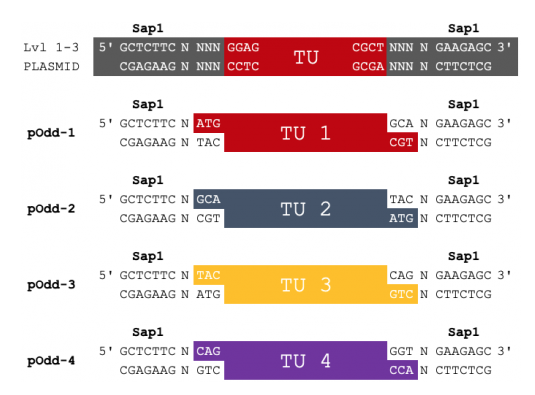
\includegraphics[width=0.8\textwidth]{images/chap4/chap4_typ_02.png}
    \label{fig:ch4typ02}
\end{figure}
\FloatBarrier
\noindent
The fusion sites on each plasmid determine the position of each TU in the final level 2 construct.\\ \\
To domesticate a part - i.e. clone it into the Universal Acceptor Vector (pSB1C00) - it must be flanked with the right vector fusion sites. The easiest way to achieve this is using extension PCR to introduce these features as prefix/suffix to the part. The next step is using SapI to clone it into pSB1C00.

\subsection*{Level 1}
The RFC 1000 Standard offers 4 level 1 plasmids, their SapI restriction sites leave 3bp fusion sites, which allow for the assembly of multi-gene units of up to 4 TUs in a level 2 assembly. This number can be expanded by creating new level 1 backbones or by performing further cloning steps after level 2. The fact that the backbones used already conform to Loop make it easy to assemble larger constructs. \\ \\
The Backbones used for level 1 plasmids are pSB1K01-pSB1K04, they are based on the pOdd backbones from the loop assembly. 

\subsection*{Level 2}
The next step is assembling TUs into a level 2 backbone to build multi-gene units (MTUs), the Type IIs standard offers four plasmids for this job, which are also based on the Loop plasmids pEven1 - pEven4. The TUs can then be assembled in level 2 plasmids using SapI. 

\epigraph{The following section was written by Yasoo Morimoto}{\textit{iGEM Marburg 2021}}
\subsection{Modular Cloning}
\noindent
Firstly introduced by \parencite{Weber2011}, the MoClo Assembly is based on the Golden Gate system \parencite{Engler2008} for building multi-gene constructs in a one step, one pot reaction. It relies on the ability of type IIs enzymes to cut outside of their recognition site to create unique and standardized overhangs. These overhangs, in turn, dictate the position of each part in the plasmid. This standard includes unique overhangs for promoters, 5’UTRs, signal peptides and more; the only two enzymes used are BsaI, Esp3I and BpiI. Plasmids code for spectinomycin, ampicillin or kanamycin \parencite{Weber2011}.

\subsubsection{Construct Design}
Transcription units (TUs) start with the promoter upstream overhang (GGAG) and end with the Terminator downstream overhang (CGCT). While restriction enzymes in level 0 plasmids have identical fusion sites, level 1 plasmids leave unique sequences after cleavage for directional cloning. The MoClo toolbox provides level 1 destination vectors with 7 different overhangs, so that one can assemble multi-gene constructs  with up to 6 TUs (positions 1 to 7) in a single reaction. This is especially attractive for creating more complicated metabolic pathways. 

\begin{figure}[!htbp]
    \centering
    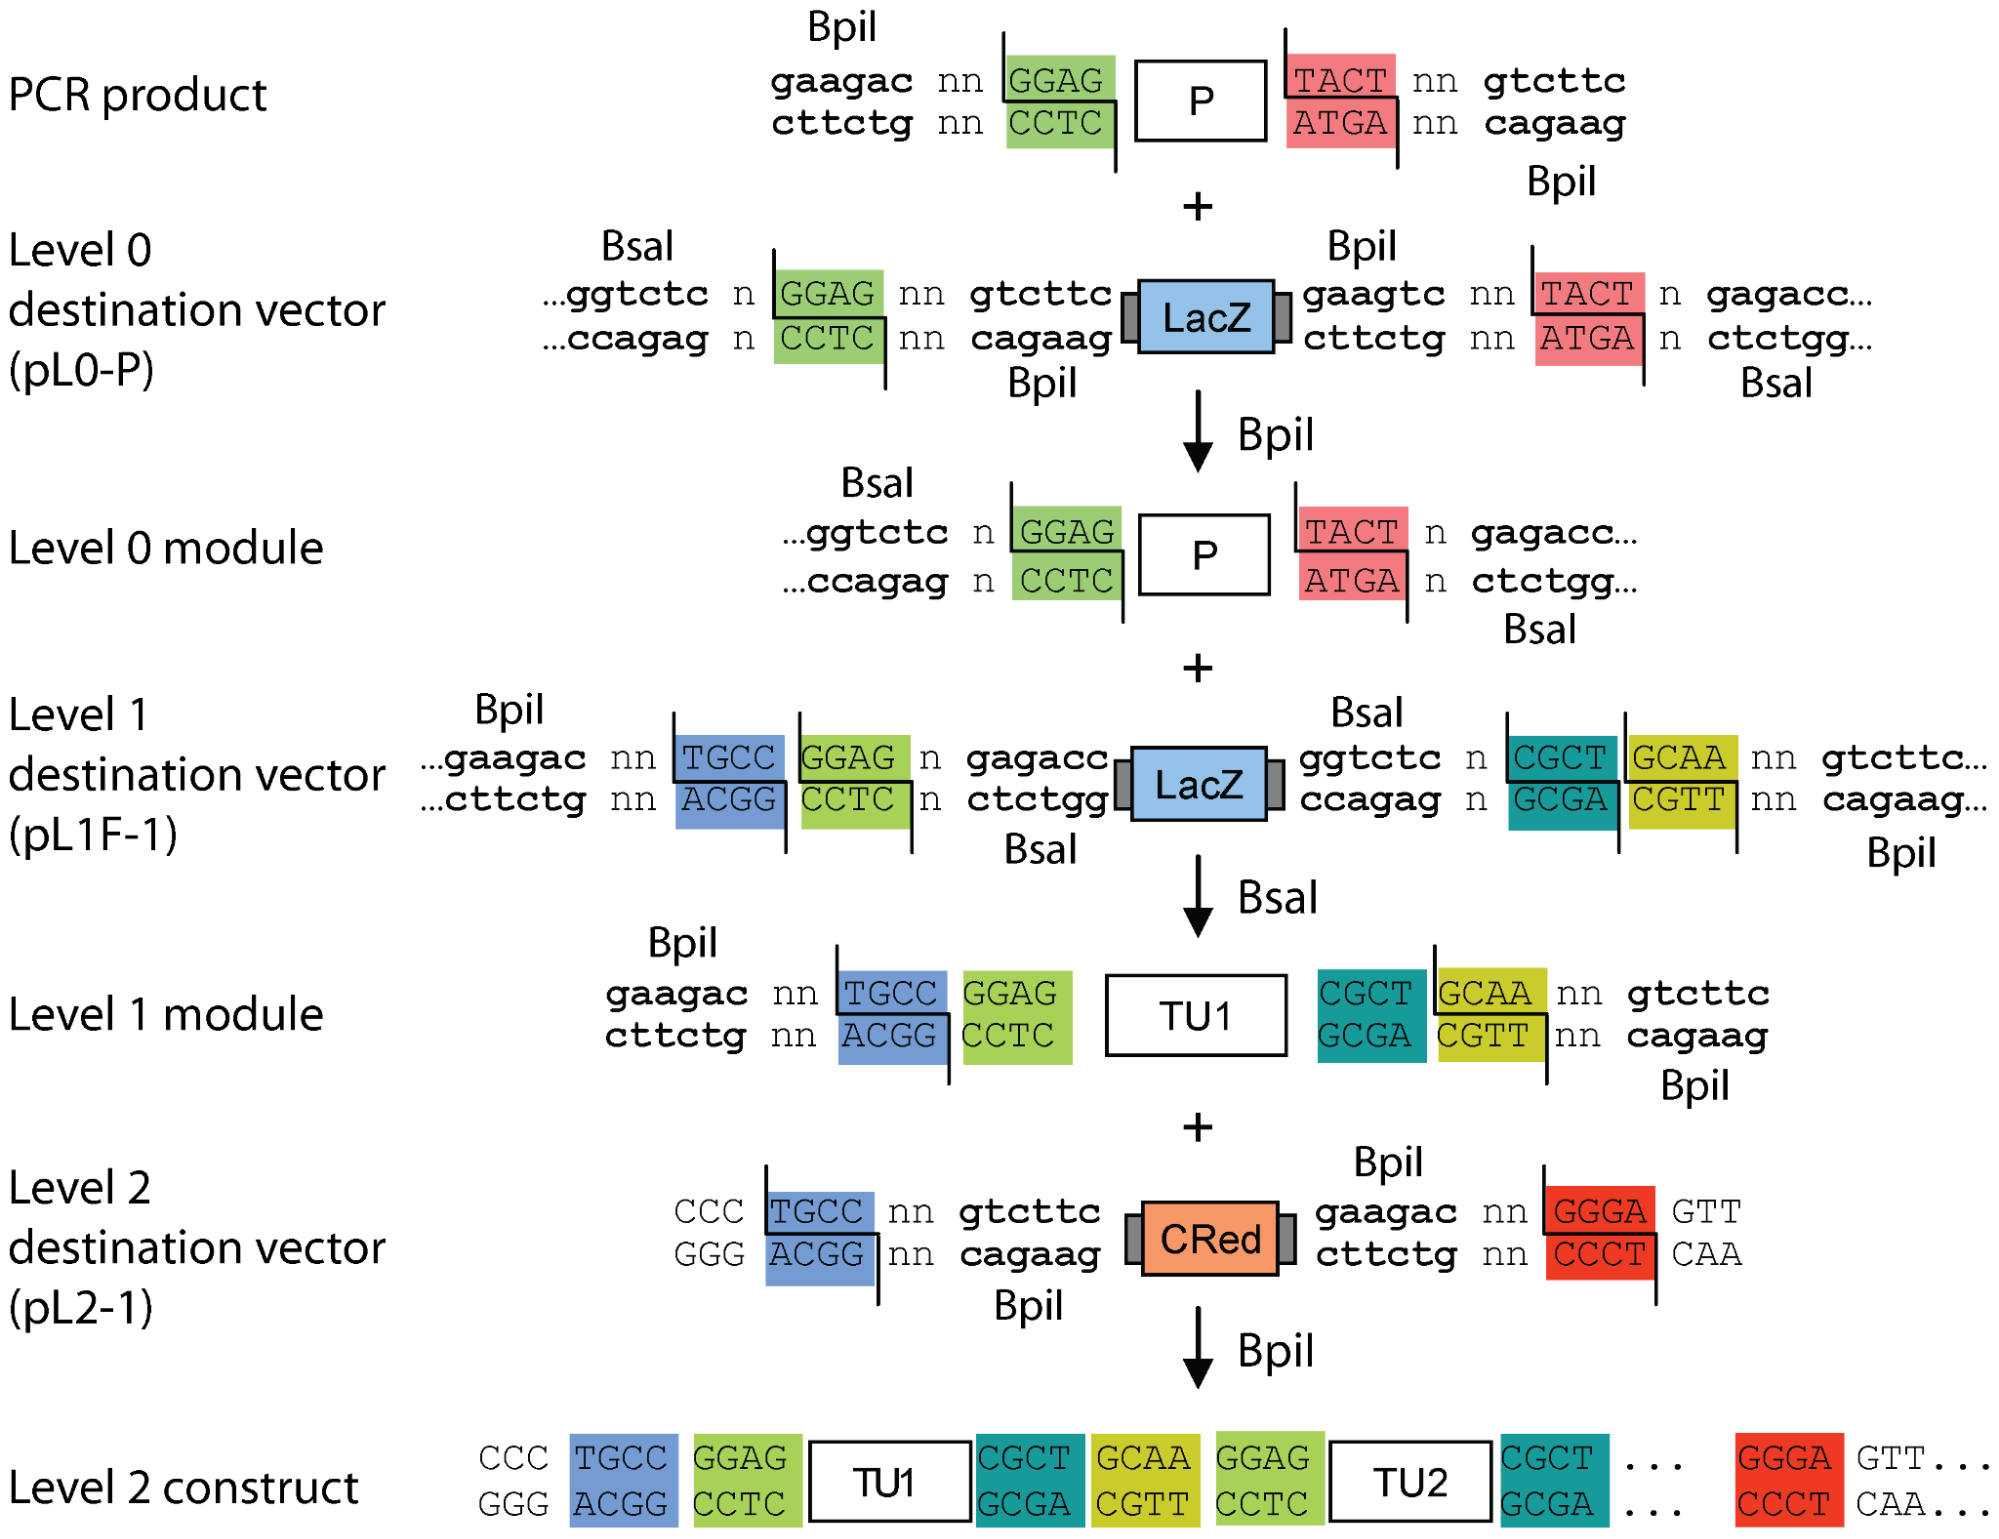
\includegraphics[width=\textwidth]{images/chap4/chap4_moclo_01.png}
    \label{fig:ch4mcl01}
\end{figure}
\FloatBarrier

\noindent The number of TUs in a level 2 plasmid is not limited to 7, though; because the fusion sites are organized in a “circular” logic, the downstream overhang at position 7 is compatible with the upstream position 1 insert. So it is theoretically possible to indefinitely extend the plasmid with new TUs by adding new reaction steps. A second set of level 1 destination plasmids allows for insertion of TUs in the reverse orientation at any position. \\ \\
To bridge the gap between the last used level 1 module (which has an variable upstream fusion site depending on its position number) and the backbone, an End Liker is required. These parts have the same selection markers as 

\epigraph{The following section was written by Yasoo Morimoto}{\textit{iGEM Marburg 2021}}
\subsection{Loop Assembly}
One of the great benefits of working with Type IIs cloning is the potential for highly standardized part design, allowing for the easy exchange between working groups. On top of this benefit, Loop Assembly \parencite{Pollak2020} also allows for an uncomplicated assembly of large constructs containing several transcription units (TUs), through recursive cloning the size of the final sequence can grow indefinitely.  Furthermore, the system is also compatible with long-overlap assembly, TUs can also be cloned using Gibson Assembly.

\subsubsection{Components}
Loop Assembly works by alternating a set of four odd number plasmids (pOdd) with a set of four even numbered plasmids (pEven). Both types of plasmids possess SapI and BsaI cutting sites, albeit in different orientations. \\ 

\textbf{pEven1 - 4}
\begin{itemize}[noitemsep,topsep=0pt]
    \item Spectinomycin
    \item SapI for cloning step
    \item LacZ Dropout
    \item UNSp1 - 5
    \item UNSx
\end{itemize} 


\textbf{pOdd1 - 4}
\begin{itemize}[noitemsep,topsep=0pt]
    \item Kanamycin
    \item BsaI for cloning step
    \item LacZ Dropout
    \item UNSp1 - 5
    \item UNSpx
\end{itemize}  


\textbf{POdd Spacer}
\begin{itemize}[noitemsep,topsep=0pt]
    \item 200bp random DNA spacer
    \item Kanamycin
    \item BsaI for cloning step
\end{itemize} 


\textbf{PEven Spacer}
\begin{itemize}[noitemsep,topsep=0pt]
    \item 200bp random DNA spacer
    \item Kanamycin
    \item SapI for cloning step
\end{itemize} 
\mbox{} \\
All plasmids contain the pMB1 origin of replication.

\subsubsection{Cloning Method}
As a MoClo Standard, Loop relies on Level 0 parts with compatible overhangs to build it’s transcription units. pOdd plasmids are receiver to level 0 parts compatible to the PhytoBricks standard \parencite{Patron2015}. Cutting them with BsaI leaves the promoter CCTC and terminator CGCT overhangs on the backbone, this allows the cloning of one TU (level 1 construct). To clone into a level 2 plasmid, four TUs cloned in pOdd1 - pOdd4 are assembled in a reaction with SapI to clone in a level 2 pEven plasmid. Each POdd plasmid defines the position of it’s TU through the fusion sites left by the SapI restriction reaction, the sites are named $\alpha, \beta, \gamma, \epsilon, \omega$, and all pEven backbones have $\alpha$ and $\omega$ fusion sites for the first and the last TUs. 

\begin{figure}[!htbp]
    \centering
    \caption{Adapted from \parencite{Pollak2020}.}
    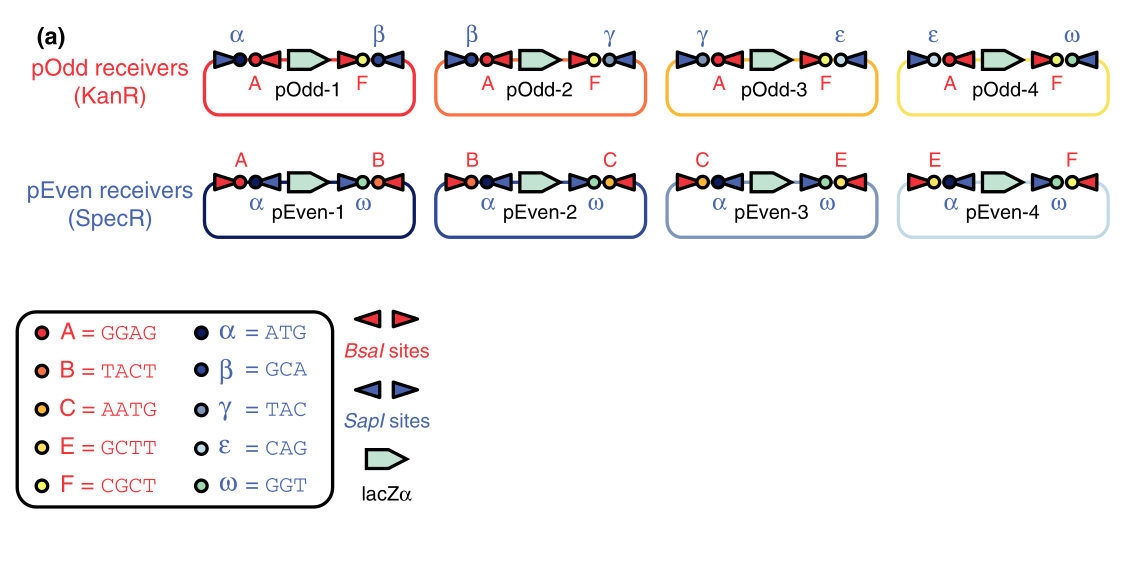
\includegraphics[width=\textwidth]{images/chap4/chap4_loop_01.png}
    \label{fig:ch4loop01}
\end{figure}
\FloatBarrier

\noindent
The important feature of Loop comes now: you can just keep going with another round of cloning. With four level 2 pEven plasmids it is possible to set up a level 3 reaction and  assemble 16 TUs in a pOdd plasmid. Here, the fusion sites left by BsaI determine the position of each insert. Because of the way the overhangs are layed out, each cloning step must introduce four inserts, this exponentially increases the amount of TUs cloned. For use-cases that need a smaller number of TUs, the system offers a “Universal Spacer” that can be cloned in any receiver plasmid, this Universal Spacer contains 200bp random DNA devoid of BsaI or SapI cutting sites. 

\begin{figure}[!htbp]
    \centering
    \caption{Adapted from (Pollak et al., 2019)}
    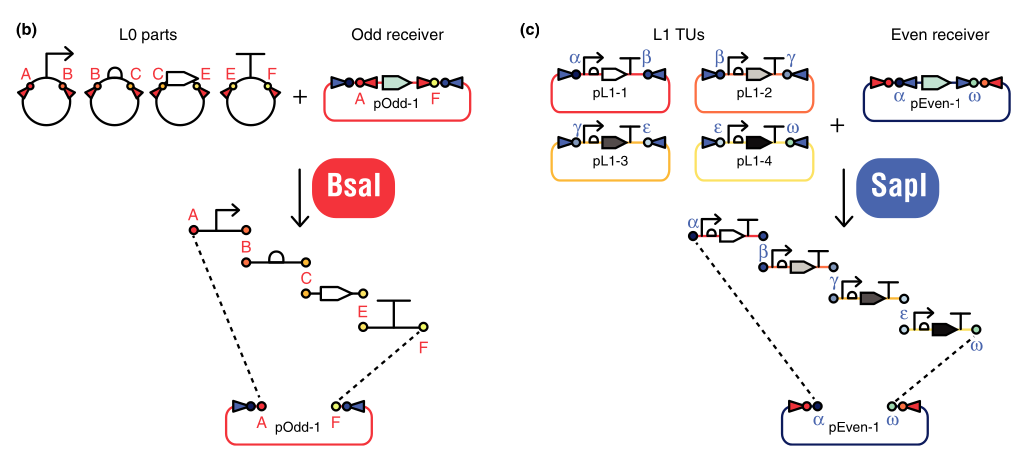
\includegraphics[width=\textwidth]{images/chap4/chap4_loop_02.png}
    \label{fig:ch4loop02}
\end{figure}
\FloatBarrier

\subsubsection{Long Overlap Assembly} 
In addition to Type IIs, long overlap assembly cloning methods have also gained popularity in the synthetic biology community. Methods like Gibson Assembly \parencite{Gibson2008} offer a low cost and fast cloning method capable of assembling several fragments in a one-pot isothermal reaction. Furthermore, new methods aim to streamline this process by introducing standardized unique nucleotide sequences (UNSs) that allow us to combine several TUs in a larger construct \parencite{Pollak2020} \parencite{Torella2013}. \\ \\
Flanking the cutting sites for BsaI and SapI, the Loop Plasmids include UNSs for the assembly of multi-gene constructs using Gibson Assembly.

\begin{figure}[!htbp]
    \centering
    \caption{Adapted from \parencite{Pollak2020}.}
    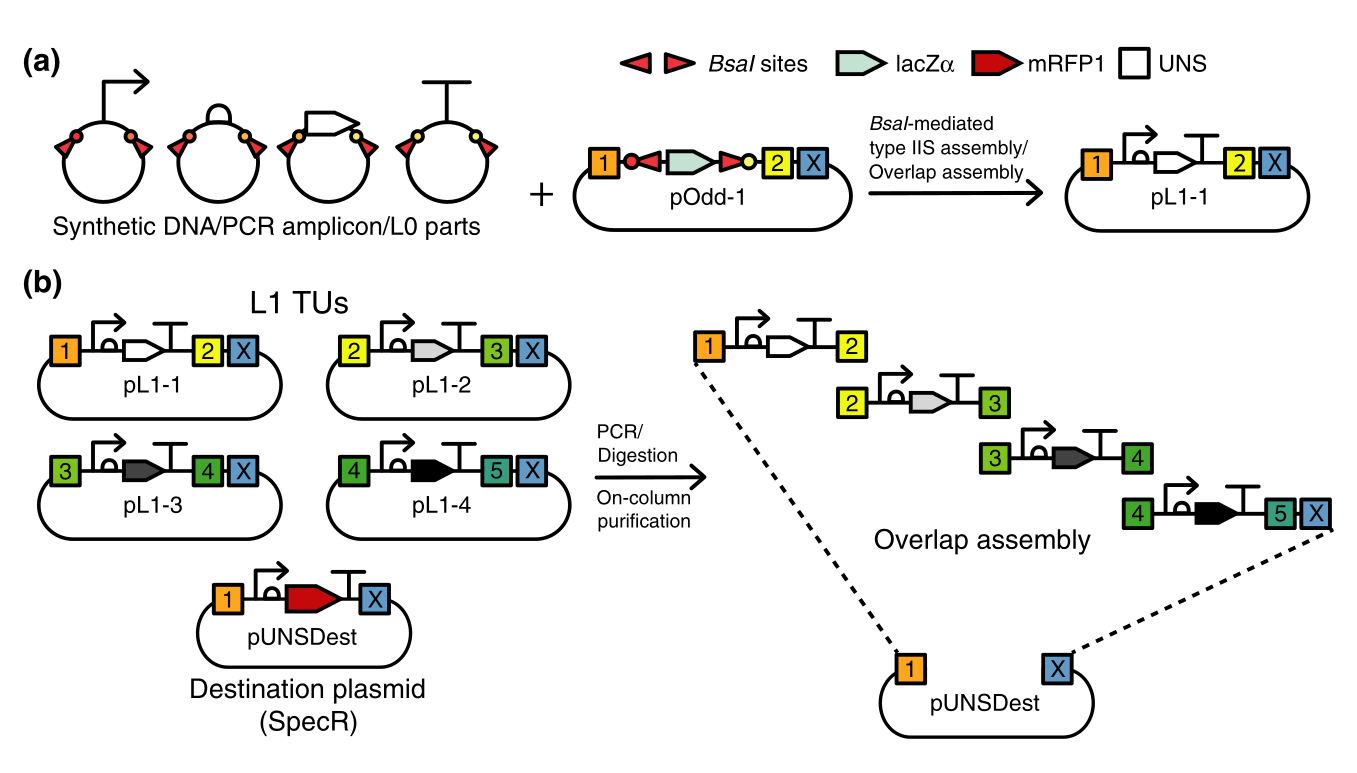
\includegraphics[width=\textwidth]{images/chap4/chap4_loop_03.png}
    \label{fig:ch4loop03}
\end{figure}
\FloatBarrier


\epigraph{The following section was written by Paul Goffing}{\textit{iGEM Bielefeld-CeBiTec 2021}}
\subsection{Mobius Assembly}
\subsubsection{Introduction}
The Mobius Assembly is a recent adaption of the Golden Gate cloning system and Modular Cloning, developed by Andreas Andreou at Naomi Nakayama’s lab \parencite{Andreou2018}. In their publication, the authors state that the Mobius Assembly makes Golden Gate more versatile without compromising capacity. In addition, especially interesting for iGEM Teams working with plants, the used backbones are binary plasmids. This means that Mobius Assembly can be used for Agrobacterium-mediated transformation of plants. The developers of Mobius Assembly expanded in their method standards which were set by iGEM: the backbones are based on the iGEM standard vectors pSB1C3 and pSB1K3 and the choice of overhangs is based on Phytobricks. Thus, Mobius Assembly is compatible with all iGEM Type IIS standard parts.\\ \\
Enzymes used: BsaI, AarI, EcoRI, PstI, T4 DNA Ligase \\
Antibiotics used: Chloramphenicol, Kanamycin, Spectinomycin
\subsubsection{Basic Principle}
The Mobius Assembly basically works like iGEM Type IIS cloning. Basic parts are assembled in Level 0 vectors (mUAV - Mobius Universal Acceptor Vector). They can be assembled to transcriptional units (TUs) in Level 1. TUs from Level 1 can be combined in Level 2. If more TUs need to be combined or added later, it is possible to switch back and forth between Level 2 and Level 1. This switching back and forth is where the name Mobius Assembly comes from. \\ \\
Let me remind you how Type IIS cloning works. Type IIS restriction enzymes recognize a specific sequence and cut at a different position, creating sticky ends. This gives the opportunity to create a large number of different overhangs by using only one restriction enzyme. At the position, where two basic parts need to be combined, they share the same overhang. At the same time, the same overhang is only used at one ligation site between basic parts. This order of different overhangs results in two things: First, all basic parts will always be assembled in the correct order. Second, basic parts are exchangeable, if they have the same overhangs. To facilitate the latter aspect, Phytobricks standardised the use of overhangs, shown in figure 1B. \\ \\
In comparison to other cloning methods, like Gibson Assembly or Biobrick standard, it is quite easy and fast to assemble large vectors containing many different basic parts using Mobius Assembly.
\subsubsection{Cloning}
If you decide to use mobius assembly, I strongly recommend to follow the instructions from this Springer protocol \parencite{Andreou2020}. \textbf{Important note}: The figure in this Springer protocol has an error! The first overhang must be GGAG and not GAAG!
\paragraph{Level 0 cloning} \mbox{}\\
The first step in Mobius Assembly is the creation of Level 0 vectors containing all the basic parts you want to use. The Level 0 empty vector is called mUAV (Mobius Universal Acceptor Vector). It has a chloramphenicol resistance and carries the amilCP gene as a negative selection marker, which gives the colonies carrying the empty vector a strong purple colour. This makes it possible to screen colonies without the use of expensive chemicals like IPTG and X-Gal for screening and also allows the use of strains which don’t have a lacZ deletion. mUAV is not a binary vector. So this vector cannot be used to transform plants via Agrobacteria.\\ \\
The cloning of your parts into mUAV is quite simple (see Figure 4.7 A: for a graphical representation).
\begin{enumerate}
\item Amplify your part using primers with overhangs, which introduce the overhangs for Level 1 cloning and the recognition sites for AarI and BsaI. Purify the PCR product.
\item Digest mUAV and your PCR product with AarI, ligate with T4 DNA Ligase (in a one pot reaction).
\item Transform the ligated plasmids into E. coli (Top10 or DH5α).
\item Control restriction digest with EcoRI and PstI.
\item Sequence positive clones (this is the only necessary sequencing step in Mobius Assembly)
\end{enumerate}

\begin{figure}[!htbp]
    \centering
    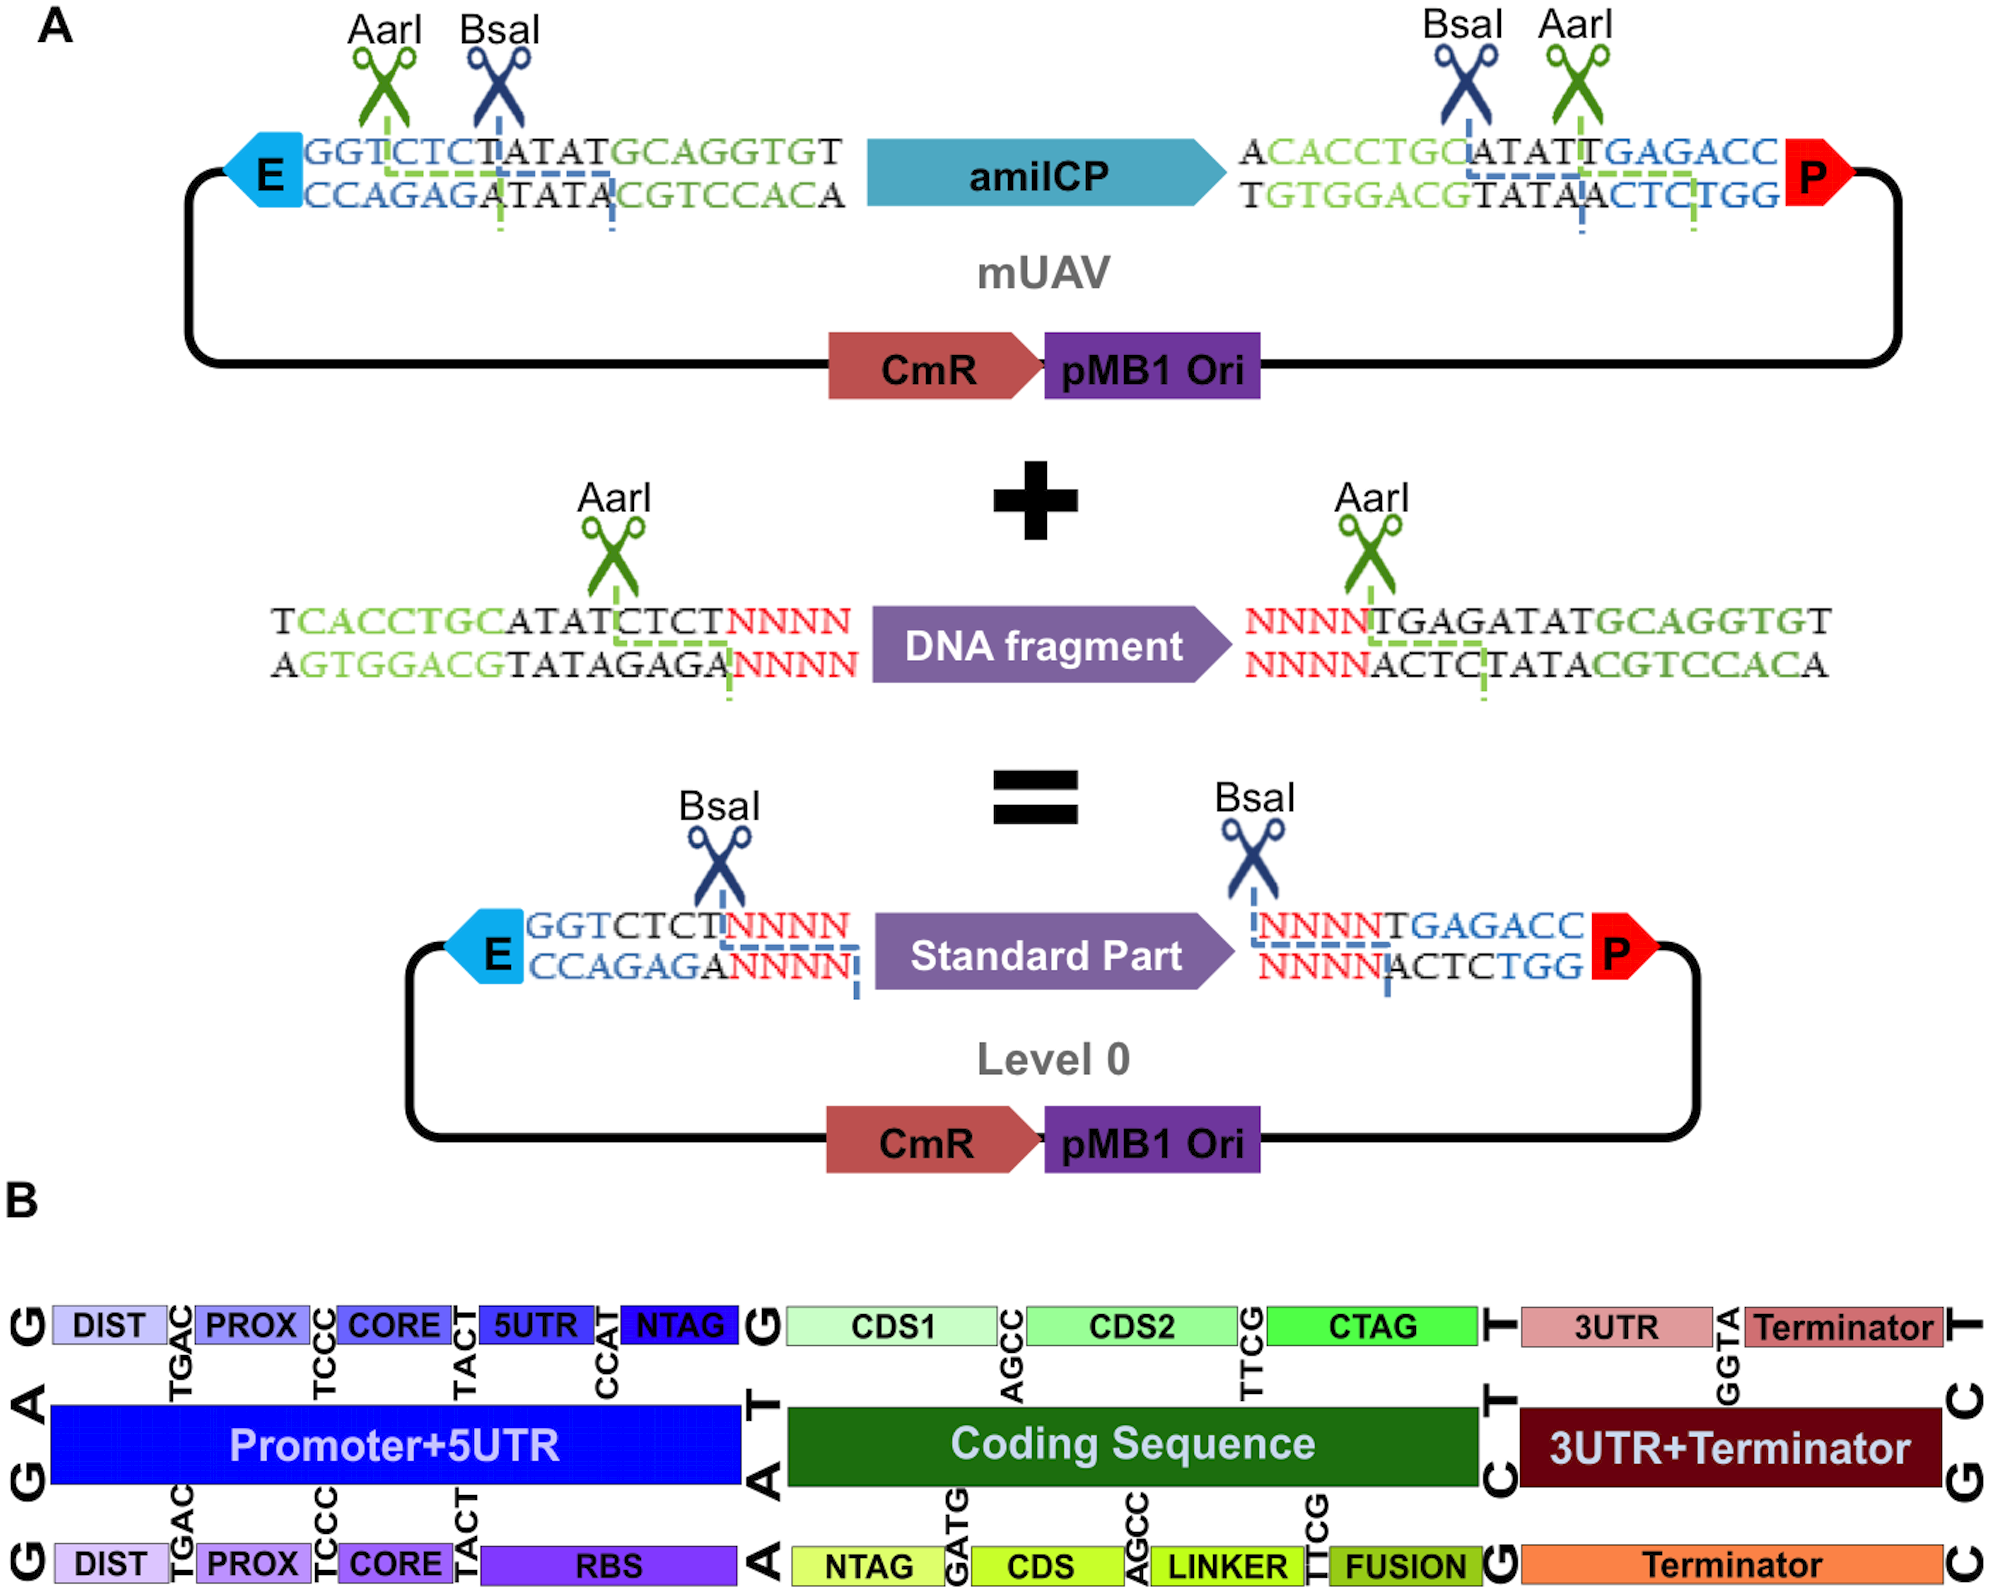
\includegraphics[width=\textwidth]{images/chap4/chap4_mob_01.png}
    \label{fig:ch4mob01}
    \caption{Adapted from \parencite{Andreou2018}.}
\end{figure}
\FloatBarrier

\paragraph{Level 1 cloning} \mbox{} \\
In Level 1, basic parts from Level 0 can be combined to form a transcriptional unit (TU). As described above, the overhangs 5’ and 3’ of the parts determine the order in which they are combined. The 5’ overhang of the promotor needs to be GGAT and the 3’ overhang of the terminator needs to be CGCT. This makes it possible to ligate the parts in Level 1. \\ \\
There are four Level 1 acceptor vectors, A, B, Γ, Δ (the greek capital letters Alpha, Beta, Gamma and Delta). One always starts with the first Level 1 acceptor vector, Level 1A. If it is necessary to assemble multiple TUs in Level 2, they will be assembled using the vectors B, Γ and Δ. \\ \\
The Level 1 vectors are based on pSB1K3. With the assembly of a TU, the spisPink gene is replaced. Thus, colonies with the empty vector are pink while colonies with vectors with insert are white. As in Level 0 cloning the spisPink works as negative selection marker. The vector carries a resistance against kanamycin.\\ \\
The cloning of Level 1 is as simple as the cloning of Level 0:
\begin{enumerate}
    \item Digestion of the Level 1 accepter vector together with all the basic parts one wants to assemble to a TU with BsaI, ligation with T4 DNA Ligase (in a one pot reaction).
    \item Transform the ligated plasmids into E. coli (Top10 or DH5α).
    \item Control restriction digest with EcoRI and PstI.
\item Sequencing of positive clones is only necessary, if Level 2 cloning fails.
\end{enumerate}
\paragraph{Level 2 cloning} \mbox{}\\
In Level 2 up to 4 TUs can be assembled to form a multi-TU-construct. If there is the need to assemble more than 4 TUs, multiple Level 2 vectors (containing multiple TUs) can be combined in Level1 afterwards. Level 2 cloning is very similar to Level 1 cloning. There are the different acceptor vectors A, B, Γ and Δ. Also, one starts assembling in the first vector, A. Level 2 requires additional auxiliary plasmids as middle-to-end-linkers or end-to-end-linkers. These auxiliary plasmids need to be added together with the Level 1 vectors to the ligation reaction. For the assembly of 4 TUs in Level 1A, the plasmid Auxiliary A needs to be added, for the assembly of 4 TUs in Level 1B, the plasmid Auxiliary B needs to be added, and so on. Additionally, there are three different middle-to-end linker auxiliary plasmids, Auxiliary 1, Auxiliary 2 and Auxiliary 3, for the assembly of 1, 2 or 3 TUs in Level 2. \\ \\
All Level 2 vectors carry a spectinomycin resistance and are again based on pSB1C3. The negative selection marker sfGFP colours the negative transformands yellow. \\ \\
\begin{enumerate}
    \item Digestion of the Level 1 accepter vector together with all the basic parts one wants to assemble to a TU and the proper auxiliary plasmid with AarI, ligation with T4 DNA Ligase (in a one pot reaction).
    \item Transform the ligated plasmids into E. coli (Top10 or DH5α).
    \item Control restriction digest with EcoRI and PstI.
\end{enumerate}
\paragraph{Primer Design} \mbox{} \\
For Level 0 cloning, the basic parts need to be inserted using specific overhangs. Also, additional recognition sequences for the Type-IIS enzymes need to be added. Therefore it is necessary to either order gene synthesis directly with the suitable overhangs or to amplify the fragment using primers with these overhangs and a proof-reading polymerase. A step-by-step introduction into primer design is also included in the Springer protocol mentioned above. This Springer protocol also explains all the other experimental procedures step-by-step. \\ \\
If the sequence you want to amplify contains recognition sites for AarI or BsaI, it is necessary to domesticate the sequence, which means to remove the recognition sites. For this, the sequence 5’ of the recognition sequence and 3’ of the recognition sequence are amplified with primers, which replace one nucleotide, so that the amino acid is still the same, but the recognition site is destroyed. There again the additional overhangs for the recognition sites of the Type-IIS enzymes are added. In the end, both PCR products are used together for Level 0 cloning.

\epigraph{The following section was written by Michael Burgis}{\textit{iGEM Marburg 2021}}
\subsection{Golden Braid}
In the beginning of the development of TypeIIS assembly strategies, the Modular Cloning standard and the Golden Braid system were designed completely independently and were published one after each other. Therefore each system has not considered the standards of the other system, which made them incompatible. 
The main features of the original Golden Braid system are that it is based on the type IIS restriction enzymes, allows the indefinite growth of reusable gene modules, consists of a set of just four destination plasmids (pDGBs) designed to incorporate multipartite assemblies made of standard DNA parts \parencite{Sarrion-Perdigones2011}.  \\ \\
In contrast to the Modular Cloning system, modules are combined \textbf{binarily} to build increasingly complex multigene constructs, \textbf{instead of the hierarchical/multipartite assembly cloning approach}. \\ \\
Nowadays the newer versions of the Golden Braid system \parencite{Sarrion-Perdigones2013} are far more used than the original, as it combines some advantages of the Modular cloning system, such as the standardized basic parts and the fast assembly of single transcription units combined with the simplicity of the original binary Golden Braid system, which just needs a few vectors, instead of a large number of acceptor vectors and end-linkers. Additionally this updated version introduced the concept of the universal acceptor vector for parts, which is also continuously used in the Phytobrick standard.

\begin{figure}[!htbp]
    \centering
    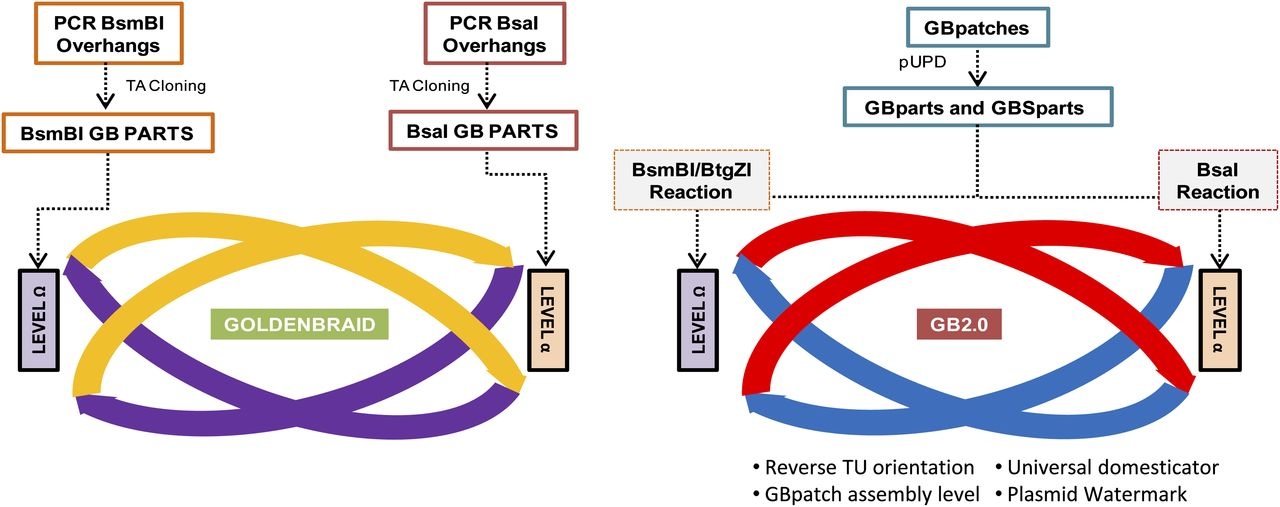
\includegraphics[width=\textwidth]{images/chap4/chap4_gb_01.png}
    \label{fig:ch4gb01}
\end{figure}
\FloatBarrier
\noindent
After building a new TU , utilizing a multipartite assembly, the resulting new transcriptional unit can be binarily combined with another transcriptional unit to produce increasingly complex multigene structures. The solution provided by GoldenBraid cloning system relies on the special design of GoldenBraid destination vectors, which introduces a double loop (braid) into the cloning strategy. A composite part (a TU or a group of TUs) cloned in a given entry vector can be combined only with a second composite part cloned in the complementary entry vectors at the same level. This is done in the presence of a destination vector of the opposite level and generates a new expression vector at the opposite level. \\ \\
Besides the most adapted Modular Cloning system, the Golden Braid system is also adapted in the plant synthetic biology community. After the introduction of the Phytobrick standard, both standards became compatible and accelerated the characterization of standardized genetic parts for plant engineering \parencite{Sarrion-Perdigones2013}.
